\documentclass[12pt]{beamer}
\usepackage{../Estilos/BeamerMAF}
\usepackage[absolute, overlay]{textpos}
\usepackage{../Estilos/ColoresLatex}
\input{../Preambulos/preambulo_Beamer_Copenhagen_wolverine}

\setbeamercolor{section in foot}{bg=regalia, fg=white}
\setbeamercolor{subsection in foot}{bg=operamauve, fg=black}

\makeatletter
\setbeamertemplate{footline}
{
\leavevmode%
\hbox{%
\begin{beamercolorbox}[wd=.333333\paperwidth,ht=2.25ex,dp=1ex,center]{section in foot}%
  \usebeamerfont{section in foot} \insertsection
\end{beamercolorbox}%
\begin{beamercolorbox}[wd=.333333\paperwidth,ht=2.25ex,dp=1ex,center]{subsection in foot}%
  \usebeamerfont{subsection in foot}  \insertsubsection
\end{beamercolorbox}%
\begin{beamercolorbox}[wd=.333333\paperwidth,ht=2.25ex,dp=1ex,right]{date in head/foot}%
  \usebeamerfont{date in head/foot} \insertshortdate{} \hspace*{1.5em}
  \insertframenumber{} / \inserttotalframenumber \hspace*{2ex} 
\end{beamercolorbox}}%
\vskip0pt%
}
\makeatother
\usefonttheme{serif}
\setbeamercolor{frametitle}{bg=olivine}
\resetcounteronoverlays{saveenumi}

\date{24 de mayo de 2022}

\title{\large{Minimizando el error de interpolación}}
\subtitle{Polinomios de Chebyshev}
\author{M. en C. Gustavo Contreras Mayén}

\begin{document}
\maketitle
\fontsize{14}{14}\selectfont
\spanishdecimal{.}

\section*{Contenido}
\frame{\frametitle{Temas a revisar} \tableofcontents[currentsection, hideallsubsections]}

%Ref. Nasini - Minimizar el error con polinomios de Chebyshev
\section{Interpolación}
\frame{\tableofcontents[currentsection, hideothersubsections]}
\subsection{Introducción}

\begin{frame}
\frametitle{Polinomio de interpolación}
Un polinomio de interpolación es un polinomio que pasa exactamente a través de un conjunto dado de puntos.
\end{frame}
\begin{frame}
\frametitle{Diferencia entre ajuste curvas e interpolación}
Ajuste por interpolación:
\begin{figure}
   \centering
   \includegraphics[scale=0.5]{Imagenes/Interpol02.eps}
\end{figure}
\end{frame}
\begin{frame}
\frametitle{Diferencia entre ajuste curvas e interpolación}
Ajuste de la curva:
\begin{figure}
   \centering
   \includegraphics[scale=0.5]{Imagenes/Interpol03.eps}
\end{figure}
\end{frame}
\begin{frame}
\frametitle{Polinomio de interpolación}
Supongamos que lo que se quiere es buscar un polinomio de grado finito que aproxime una función dada.
\\
\bigskip
\pause
Lo que resulta intuitivo es buscar que dicho polinomio tenga el mismo valor de la función en un conjunto de puntos dado.
\end{frame}
\begin{frame}
\frametitle{Polinomio de interpolación}
Sabiendo que por $n$ puntos pasa un único polinomio de grado $n-1$, podríamos argumentar que la única manera de buscar una aproximación mejor del polinomio a la función es la de escoger de formas distintas los puntos por los cuales el polinomio ha de pasar.
\end{frame}
\begin{frame}
\frametitle{Polinomio de interpolación}
Dada una función $f(x)$ de la cual se conocen sus valores en un número finito de puntos $x_{0}, x_{1}, \ldots, x_{m}$, \pause se llama \textbf{\textcolor{red(ncs)}{interpolación polinómica}} al proceso de hallar un polinomio $p_{m}(x)$ de grado menor o igual a $m$, cumpliendo $p_{m}(x_{k}) = f(x_{k})$ parar cada $k = 1, 2, \ldots, m$.
\end{frame}
\begin{frame}
\frametitle{Polinomio de interpolación}
Los coeficientes $a_{0}, a_{1}, a_{2}, \ldots, a_{n}$, de dicho polinomio se obtienen imponiendo al polinomio de pasar por los puntos experimentales.
\end{frame}
\begin{frame}
\frametitle{Sistema matricial}
\begin{align*}
\mqty[
x_{0}^{n} & x_{0}^{n-1} & x_{0}^{n-2} & \ldots & x_{0} & 1 \\
x_{1}^{n} & x_{1}^{n-1} & x_{1}^{n-2} & \ldots & x_{1} & 1 \\
\vdots & \vdots & \vdots & & \vdots & \vdots \\
x_{n}^{n} & x_{n}^{n-1} & x_{n}^{n-2} & \ldots & x_{n} & 1 
]
\mqty[
a_{n} \\ a_{n-1} \\ \vdots \\ a_{0}
]
=
\mqty[
y_{0} \\ y_{1} \\ \vdots \\ y_{n}
]
\end{align*}
\pause
Este sistema es compatible y a la matriz asociada se le suele denominar \textbf{\textcolor{richblack}{matriz de Vandermonde}}.
\end{frame}
\begin{frame}
\frametitle{Complejidad computacional}
La complejidad computacional para invertir la matriz es de $\order{n^{3}}$.
\\
\bigskip
\pause
Por esta razón, han sido construidos diferentes algoritmos que aprovechan la particular estructura de este sistema que reducen la complejidad a $\order{n^{2}}$, \pause como el \textbf{\textcolor{riflegreen}{método de Lagrange}} \pause o el \textbf{\textcolor{rosewood}{método de las diferencias divididas de Newton}}.
\end{frame}

\section{Interpolación de Lagrange}
\frame{\tableofcontents[currentsection, hideothersubsections]}
\subsection{El método de interpolación}

\begin{frame}
\frametitle{El método de Lagrange}
El polinomio interpolador de grado $n$ de Lagrange es un polinomio de la forma:
\pause
\begin{align*}
p_{n} (x) = \nsum_{j=0}^{k} f_{j} (x) \, l_{j} (x) \hspace{1.5cm} n \leq m
\end{align*}
\end{frame}
\begin{frame}
\frametitle{Polinomios de Lagrange}
Donde los $l_{j}(x)$ son los llamados \emph{polinomios de Lagrange}, que se calculan como:
\pause
\fontsize{12}{12}\selectfont
\begin{eqnarray*}
\begin{aligned}
&l_{j}(x) = \prod_{j \neq i} \dfrac{x - x_{i}}{x_{j} - x_{i}} = \\[0.5em] \pause
&= \dfrac{(x {-} x_{0})(x {-} x_{i}) \ldots(x {-} x_{j-1})(x {-} x_{j+1}) \ldots (x {-} x_{n})}{(x_{j} {-} x_{0})(x_{j} {-} x_{1}) \ldots(x_{j} {-} x_{j-1})(x_{j} {-} x_{j+1}) \ldots (x_{j} {-} x_{n})}
\end{aligned}
\end{eqnarray*}
\end{frame}
\begin{frame}
\frametitle{Ejemplo}
Se quiere hallar el valor de la función:
\pause
\begin{align*}
f (x) = e^{x+1}
\end{align*}
Utilizando un polinomio de interpolación de Lagrange de grado $2$ que pase por los puntos:
\pause
\fontsize{12}{12}\selectfont
\begin{table}
\centering
\begin{tabular}{c | c}
$x$ & $f(x)$ \\ \hline
$0$ & $f(0)$ \\
$0.5$ & $f(0.5)$ \\
$1$ & $f(1)$ \\
\end{tabular}
\end{table}
\end{frame}
\begin{frame}
\frametitle{Gráfica de los puntos}
Al graficar los puntos tendremos lo siguiente:
\begin{figure}
   \centering  
   \includegraphics[scale=0.95]{Imagenes/Plot_Chebyshev_Ejercicio_Interp_01.eps}
\end{figure}
\end{frame}
\begin{frame}
\frametitle{Obteniendo los polinomios}
Usamos el método directo para calcular el polinomio de interpolación. \pause Con las condiciones dadas, los polinomios de Lagrange son:
\pause
\begin{eqnarray*}
\begin{aligned}
l_{0} (x) &= \dfrac{(x - 0.5)(x - 1)}{0.5} = \pause 2 \, x^{2} - 3 \, x + 1 \\[0.5em] \pause 
l_{1} (x) &= \dfrac{x (x - 1)}{-0.25} = \pause - 4 \, x^{2} + 4 \, x \\[0.5em] \pause
l_{2} (x) &= \dfrac{x (x - 0.5)}{0.5} = \pause 2 \, x^{2} - x
\end{aligned}
\end{eqnarray*}
\end{frame}
\begin{frame}
\frametitle{Polinomio de interpolación}
El polinomio de interpolación de Lagrange de grado $2$ es:
\pause
\begin{eqnarray*}
\begin{aligned}
p_{2} (x) &= \nsum_{j=0}^{2} f_{j}(x) \, l_{j}(x) = \\[0.5em] \pause
&= (2 \, e - 4 \, e^{3/2} + 2 \, e^{2}) \, x^{2} + \\[0.5em]
&+ (-3 \, e \, + 4 \, e^{3/2} + 2 \, e^{2}) \, x + e
\end{aligned}
\end{eqnarray*}
\end{frame}
\begin{frame}
\frametitle{Comparando el resultado}
\begin{figure}
    \centering
    \includegraphics[scale=0.81]{Imagenes/Plot_Chebyshev_Ejercicio_Interp_02.eps}
\end{figure}
\end{frame}
\begin{frame}
\frametitle{Error de la aproximación}
Una pregunta que puede surgir al utilizar un polinomio de interpolación para aproximar una función es qué tan bueno es el ajuste del polinomio a la función originaria.
\end{frame}
\begin{frame}
\frametitle{Error de la aproximación}
Por esta razón consideramos el error de interpolación de un polinomio de grado $n$ que pase por los puntos de una función $f(x)$ en los puntos $x_{0}, \ldots, x_{n}$.
\end{frame}
\begin{frame}
\frametitle{Error de la aproximación}
Si $f(x)$ es una función determinada en $x_{0}, \ldots, x_{n}$ y es $n$ veces diferenciable, entonces el \emph{error de interpolación} puede calcularse como valor absoluto de la diferencia entre la función y el polinomio.
\end{frame}
\begin{frame}
\frametitle{Error de la aproximación}
Construimos una función $\phi(x)$ por la cual se cumpla que:
\pause
\begin{align*}
&\phi(x) = f(x) {-} p_{n}(x) {-} a(x)(x {-} a_{0})(x {-} a_{1}) \ldots (x {-} a_{n}) \\[0.5em]
&\exists \, \bar{x} \in [-1, 1] \\[0.5em]
&a(\bar{x}) = \big[ f(x) {-} p_{n} \big] (x {-} a_{0})(x {-} a_{1}) \ldots (x {-} a_{n}) = 0
\end{align*}
\end{frame}
\begin{frame}
\frametitle{Error de interpolación}
Esta función se anula en $n + 2$ puntos. 
\\
\bigskip
\pause
Aplicando el \emph{teorema de Rolle} se tiene que una función que toma el mismo valor $n + 2$ veces tiene $n + 1$ puntos que anulan la derivada.
\end{frame}
\begin{frame}
\frametitle{Error de interpolación}
A la vez, la derivada de esta función es tal que, teniendo $n + 1$ puntos con el mismo valor tendrá $n$ puntos que anulan su derivada. 
\end{frame}
\begin{frame}
\frametitle{Error de interpolación}
Por lo tanto, derivando sucesivamente $n + 1$ veces, tenemos que existirá un único punto $\zeta$ que anule la derivada $n+1$-ésima, es decir:
\pause
\begin{align*}
\phi^{n+1} \, (\zeta) = 0
\end{align*}
\end{frame}
\begin{frame}
\frametitle{Error de interpolación}
Así podemos asegurar que $\phi^{n+1}$ tiene al menos una raíz, \pause con lo cual resulta evidente que, siendo $p_{n}(x)$ un polinomio de grado mayor que $n - 1$, $\phi^{n+1} \, (\zeta)$ resultará la siguiente:
\pause
\begin{align*}
\phi^{n+1} \, (x) = f^{(n+1)} \, (\bar{x}) - a (\bar{x}) (n + 1)!
\end{align*}
\end{frame}
\begin{frame}
\frametitle{Error de interpolación}
Por consiguiente, al haber dejado que en $\phi^{n+1} \, (\bar{x}) = 0$, se tiene que:
\pause
\begin{align*}
a (\bar{x}) = \dfrac{f^{(n+1)} \, (\bar{x})}{(n + 1)!}
\end{align*}
\end{frame}
\begin{frame}
\frametitle{Error de interpolación}
En el caso de que $f(x)$ sea $n$ veces diferenciable en el dominio $[-1, 1]$, el error de interpolación podrá definirse como:
\pause
\begin{align*}
f(x) - p_{n}(x) = \dfrac{f^{(n+1)}(\xi)}{(n + 1)!} \, \prod_{i} (x - x_{i})
\end{align*}
\pause
Donde $\xi$ es un punto que pertenece a $[-1, 1]$, por lo cual $\phi^{(n+1)}(\zeta) = 0$.
\end{frame}
\begin{frame}
\frametitle{Maximizando la expresión}
Adjudicando valores absolutos en la expresión del error de interpolación y maximizando ambos lados de la desigualdad a lo largo del intervalo $[-1, 1]$ obtenemos la cota para dicho error:
\pause
\begin{eqnarray*}
\begin{aligned}
&\max_{\abs{x} < 1} \abs{f(x) - p_{n}(x)} = \pause \abs{\dfrac{f^{(n+1)}(\xi)}{(n + 1)!} \, \prod_{i} (x - x_{i})} \leq \\[0.5em] \pause
&\leq \dfrac{\displaystyle \max_{\abs{x} < 1} \abs{f^{(n+1)}(\xi)}}{(n+1)!} \, \max_{\abs{x} < 1} \prod_{i} (x - x_{i})
\end{aligned}
\end{eqnarray*}
\end{frame}
\begin{frame}
\frametitle{Resultado del error}
Dada la unicidad del polinomio de interpolación, las únicas dos cosas que podemos mover a la hora de reducir el error de interpolación son:
\setbeamercolor{item projected}{bg=yellow,fg=black}
\setbeamertemplate{enumerate items}{%
\usebeamercolor[bg]{item projected}%
\raisebox{1.5pt}{\colorbox{bg}{\color{fg}\footnotesize\insertenumlabel}}%
}
\begin{enumerate}[<+->]
\item El grado del polinomio (por consiguiente, el número de puntos)
\item La localización de dichos puntos.
\end{enumerate}
\end{frame}
\begin{frame}
\frametitle{Resultado del error}
Se podría creer que al aumentar el grado del polinomio el error de interpolación se reduzca. 
\\
\bigskip
\pause
En realidad, pese al ser un resultado antiintuitivo, Carle David Tolmé Runge observó que el error de interpolación en un intervalo dado, tiende a infinito cuando el grado del polinomio de interpolación tiende a infinito.
\end{frame}
\begin{frame}
\frametitle{Resultado del error}
Es decir:
\pause
\begin{align*}
\lim_{n \to \infty} \big( \max_{\abs{x} < 1} \abs{f(x) - p_{n}(x)} \big) = \infty
\end{align*}
\end{frame}
\begin{frame}
\frametitle{Error mínimo}
El método que veremos nos permite proporcionar los puntos por los cuales hacer pasar el polinomio de interpolación de forma tal que la distancia máxima entre el polinomio interpolado y la función originaria sea mínima.
\end{frame}
\begin{frame}
\frametitle{Error mínimo}
La oscilación observada por Runge se puede minimizar usando nodos de Chebyshev en lugar de nodos equidistantes.
\\
\bigskip
\pause
En este caso se garantiza que el error máximo disminuye al crecer el orden polinómico.
\end{frame}

\section{Polinomios de Chebyshev}
\frame{\tableofcontents[currentsection, hideothersubsections]}
\subsection{Usando las raíces}

\begin{frame}
\frametitle{Raíces de los polinomios}
Esta es una propiedad que hace particularmente interesante el utilizar las raíces de los polinomios de Chebyshev como puntos por donde interpolar el polinomio.
\end{frame}
\begin{frame}
\frametitle{Minimizando el error}
Para minimizar el último factor de la cota del error, Pafnuty Lvovich Chebyshev demostró que los puntos $x_{0}, \ldots, x_{n}$ por los cuales hacer pasar el polinomio, han de ser escogidos de forma que:
\pause
\begin{align*}
\max_{\abs{x}<1} \prod_{i} (x - x_{i}) = \dfrac{1}{2^{n}} \, T_{n+1} (x)
\end{align*}
donde $T_{n+1}(x)$ es el polinomio de Chebyshev de primera clase de orden $n + 1$.
\end{frame}
\begin{frame}
\frametitle{Elección de los puntos}
Entre todas las elecciones de los puntos $x_{0}, \ldots, x_{n}$, elegirlos de forma que la siguiente expresión se respete:
\pause
\begin{align*}
\phi^{n+1} \, (x) = f^{(n+1)} \, (\bar{x}) - a (\bar{x}) (n + 1)!
\end{align*}
\end{frame}
\begin{frame}
\frametitle{Elección de los puntos}
Se garantiza que el polinomio así obtenido es el polinomio único que tenga la propiedad:
\pause
\begin{eqnarray*}
\begin{aligned}
\max_{\abs{x}<1} T_{n} (x) &\leq \max_{\abs{x}<1} \prod (x - x_{i}) \\[0.5em] \pause
\max_{\abs{x}<1} T_{n} (x) &= \dfrac{1}{2^{n}} \\[0.5em]
\dfrac{1}{2^{n}} &\leq \max_{\abs{x}<1} T_{n} (x)
\end{aligned}
\end{eqnarray*}
\end{frame}
\begin{frame}
\frametitle{Error de interpolación}
Se puede demostrar que el valor absoluto de la diferencia entre la función y el polinomio interpolado por las raíces del polinomio de Chebyshev resulta acotado de la siguiente forma:
\pause
\begin{align*}
\abs{f(x) - p_{n-1}} \leq \dfrac{1}{2^{n-1} \, n!} \, \max_{\xi \in [-1, 1]}  \, \abs{f^{n} \, (\xi)}
\end{align*}
\end{frame}

\section{Las raíces de Chebyshev}
\frame{\tableofcontents[currentsection, hideothersubsections]}
\subsection{Interpretación geométrica}

\begin{frame}
\frametitle{Raíces del polinomio Chebyshev}
Una interpretación geométrica de las raíces de Chebyshev es aquella según la cual estos se colocan en un segmento de longitud igual al diámetro de un círculo, cuya circunferencia repartimos en $n$ partes iguales.
\end{frame}
\begin{frame}
\frametitle{Raíces del polinomio Chebyshev}
Proyectando a lo largo del dicho segmento el punto medio de cada partición de la semicirconferencia obtenemos puntos que coinciden con las raíces del polinomio de Chebyshev.
\begin{figure}
    \centering
    \includegraphics[scale=1]{Imagenes/Nodos_Chebychev_01.eps}
\end{figure}
\end{frame}
\begin{frame}
\frametitle{Minimizando el efecto Runge}
La razón por la cual la aproximación de una función $f (x)$ por un polinomio que interpole puntos escogidos de esta forma minimiza el efecto Runge, \pause es que la densidad de puntos resulta creciente desde el centro hasta las extremidades.
\end{frame}
\begin{frame}
\frametitle{Minimizando el efecto Runge}
Para calcular dichas raíces utiliza la identidad trigonométrica del polinomio de Chebyshev:
\pause
\begin{align*}
T_{n}(x) = \cos (n \, \arccos x) = \cosh (n \, \mbox{arccosh} \, x)
\end{align*}
\pause
Este coseno se anula cuando la expresión al interior es un múltiplo de $2 \, \pi$.
\end{frame}
\begin{frame}
\frametitle{Raíces polinomio Chebyshev}
Por lo tanto las raíces del polinomio de Chebyshev en $[-1, 1]$ son:
\pause
\begin{align*}
x_{i} = \cos \left( \dfrac{2 \, i - 1}{2 \, n} \, \pi \right) \hspace{1cm} i = 1, 2, \ldots, n
\end{align*}
\end{frame}
\begin{frame}
\frametitle{Raíces polinomio Chebyshev}
En el caso de que se quisiera definir el polinomio de Chebyshev en un intervalo cualquiera $[a, b]$, las raíces se trasforman como:
\pause
\begin{align*}
x_{i} = \dfrac{a + b}{2} &+ \dfrac{b - a}{2} \, \cos \left( \dfrac{2 \, i - 1}{2 \, n} \, \pi \right) \\[0.5em] 
i =& 0, 1, \ldots, n
\end{align*}
\end{frame}
\begin{frame}
\frametitle{Obteniendo coeficientes}
La utilización de los nodos de Chebyshev nos permite también utilizar un método recursivo para la obtención de los coeficientes:
\pause
\begin{align*}
f(x) \simeq \sum_{j=0}^{n} c_{j} \, T_{j}(x)
\end{align*}
donde los coeficientes $c_{j}$ son:
\end{frame}
\begin{frame}
\frametitle{Obteniendo coeficientes}
Los coeficientes $c_{j}$ son:
\pause
\begin{align*}
c_{0} &= \dfrac{1}{n + 1} \, \sum_{j=0}^{n} f(x_{k}) \, T_{0}(x_{k}) = \dfrac{1}{n + 1} \, \sum_{j=0}^{n} f(x_{k}) \\[0.5em]
c_{j} &= \dfrac{1}{n + 1} \, \sum_{j=0}^{n} f(x_{k}) \, T_{j}(x_{k})
\end{align*}
\end{frame}
\begin{frame}
\frametitle{Usando los coeficientes}
Esta fórmula permita calcular los coeficientes del polinomio de interpolación con un costo computacional del orden de $\order{n^{2}}$ operaciones.
\end{frame}

\section{Ejercicio}
\frame{\tableofcontents[currentsection, hideothersubsections]}
\subsection{Ajuste polinomial}

\begin{frame}
\frametitle{Enunciado}
Consideramos la función:
\begin{align*}
f(x) = \dfrac{800 \, x}{54 \, x^{4} + x^{2} + 3}
\end{align*}
para interpolar dos polinomios de igual grado a los puntos de dicha función, en el intervalo $[-1, 1]$.
\end{frame}
\begin{frame}
\frametitle{Gráfica de la función}
La función a interpolar es la siguiente:
\begin{figure}
    \centering
    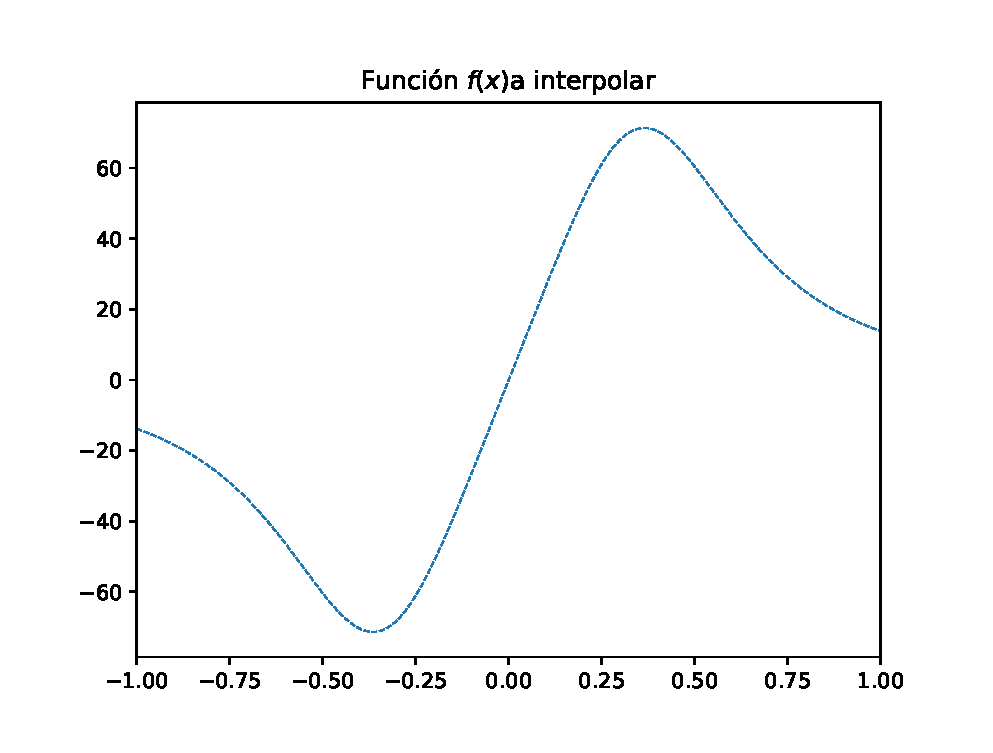
\includegraphics[scale=0.5]{Imagenes/Plot_Ejercicio_Chebychev_01.eps}
\end{figure}
\end{frame}
\begin{frame}
\frametitle{Estrategia} 
El primer polinomio lo interpolamos con puntos equidistantes y el segundo con las raíces del polinomio de Chebyshev.
\\
\bigskip
\pause
Utilizamos dos medidas de distancia para evaluar la bondad de la aproximación:
\end{frame}
\begin{frame}
\frametitle{Evaluando la aproximación}
El error debido a la diferencia del área al cuadrado entre la función y el polinomio de interpolación:
\pause
\begin{align*}
d_{1} (f, p) = \scaleint{6ex}_{\bs a}^{b} \big[ f(x) - p(x) \big]^{2} \dd{x}
\end{align*}
\end{frame}
\begin{frame}
\frametitle{Segundad medida de aproximación}
La segunda medida para medir la bondad de la aproximación es la distancia máxima entre los puntos entre la función y el polinomio de interpolación:
\pause
\begin{align*}
d_{2} (f, p) = \max_{x} \abs{f(x) - p(x)}
\end{align*}
\end{frame}

\section{Implementación con python}
\frame{\tableofcontents[currentsection, hideothersubsections]}
\subsection{Usando las librerías de python}

\begin{frame}
\frametitle{Usando python}
Con la finalidad de ocupar un lenguaje más versátil para resolver el ejercicio, usamos \textcolor{blue}{\texttt{python}} y las librerías con las cuales podremos obtener los valores de $d_{1}$ y $d_{2}$.
\end{frame}
\begin{frame}
\frametitle{Usando python}    
También con \textcolor{blue}{\texttt{python}} se elaboraron las gráficas de los procesos de aproximación con los puntos equidistantes y con los puntos de las raíces de los polinomios de Chebyshev.
\end{frame}
\begin{frame}
\frametitle{Librerías}
Se han ocupado las siguientes librerías:
\setbeamercolor{item projected}{bg=yellow,fg=black}
\setbeamertemplate{enumerate items}{%
\usebeamercolor[bg]{item projected}%
\raisebox{1.5pt}{\colorbox{bg}{\color{fg}\footnotesize\insertenumlabel}}%
}
\begin{enumerate}[<+->]
\item \texttt{numpy.polyfit} y \texttt{numpy.poly1d}.
\item \texttt{scipy.integrate.quad}
\item \texttt{scipy.special.roots\_chebyt}
\item \texttt{matplotlib.pyplot}
\end{enumerate}
\end{frame}

\subsection{Obteniendo las aproximaciones}

\begin{frame}
\frametitle{Resolviendo el problema}
Se calculan $d_{1}$, $d_{2}$, así como las gráficas del ajuste polinomial con puntos equidistantes y con las raíces del polinomio de Chebyshev para el conjunto de puntos:
\pause
\begin{align*}
n = 3, 5, 8, 10, 12, 14, 16
\end{align*}
que se presentan a continuación:
\end{frame}
\begin{frame}
\frametitle{Con $n = 3$}
    \centering
    \includegraphics<1>[scale=0.6]{Imagenes/Interpolacion_Chebychev_03_Polinomio.eps}% 
    \includegraphics<2>[scale=0.6]{Imagenes/Interpolacion_Chebychev_03_Raices.eps}
\end{frame}
\begin{frame}
\frametitle{Con $n = 5$}
    \centering
    \includegraphics<1>[scale=0.6]{Imagenes/Interpolacion_Chebychev_05_Polinomio.eps}% 
    \includegraphics<2>[scale=0.6]{Imagenes/Interpolacion_Chebychev_05_Raices.eps}
\end{frame}
\begin{frame}
\frametitle{Con $n = 8$}
    \centering
    \includegraphics<1>[scale=0.6]{Imagenes/Interpolacion_Chebychev_08_Polinomio.eps}% 
    \includegraphics<2>[scale=0.6]{Imagenes/Interpolacion_Chebychev_08_Raices.eps}
\end{frame}
\begin{frame}
\frametitle{Con $n = 10$}
    \centering
    \includegraphics<1>[scale=0.6]{Imagenes/Interpolacion_Chebychev_10_Polinomio.eps}% 
    \includegraphics<2>[scale=0.6]{Imagenes/Interpolacion_Chebychev_10_Raices.eps}
\end{frame}
\begin{frame}
\frametitle{Con $n = 12$}
    \centering
    \includegraphics<1>[scale=0.6]{Imagenes/Interpolacion_Chebychev_12_Polinomio.eps}% 
    \includegraphics<2>[scale=0.6]{Imagenes/Interpolacion_Chebychev_12_Raices.eps}
\end{frame}
\begin{frame}
\frametitle{Con $n = 14$}
    \centering
    \includegraphics<1>[scale=0.6]{Imagenes/Interpolacion_Chebychev_14_Polinomio.eps}% 
    \includegraphics<2>[scale=0.6]{Imagenes/Interpolacion_Chebychev_14_Raices.eps}
\end{frame}
\begin{frame}
\frametitle{Con $n = 16$}
    \centering
    \includegraphics<1>[scale=0.6]{Imagenes/Interpolacion_Chebychev_16_Polinomio.eps}% 
    \includegraphics<2>[scale=0.6]{Imagenes/Interpolacion_Chebychev_16_Raices.eps}
\end{frame}
\begin{frame}
\frametitle{Resumen}
\begin{table}
    \fontsize{12}{12}\selectfont
\begin{tabular}{| c | c | c |} \hline
puntos & $d_{1}$ & $d_{2}$ \\\hline
\multirow{2}{*}{$3$} & $3281.06$ & $66.33$ \\
 & $2799.63$ & $62.98$ \\ \hline
 \multirow{2}{*}{$5$} & $709.14$ & $28.11$ \\
 & $714.92$ & $34.66$ \\ \hline 
 \multirow{2}{*}{$8$} & $19.85$ & $5.68$ \\
 & $6.82$ & $4.12$ \\ \hline
\end{tabular}
\end{table}
\end{frame}
\begin{frame}
\frametitle{Resumen}
\begin{minipage}[t]{0.4\textwidth}
\begin{table}
\renewcommand{\arraystretch}{0.99}
\fontsize{12}{12}\selectfont
\begin{tabular}{| c | c | c |} \hline
puntos & $d_{1}$ & $d_{2}$ \\\hline
\multirow{2}{*}{$10$} & $317.75$ & $37.95$ \\
    & $6.99$ & $3.82$ \\ \hline
    \multirow{2}{*}{$12$} & $478.56$ & $52.64$ \\
    & $3.0$ & $2.31$ \\ \hline 
    \multirow{2}{*}{$14$} & $164.88$ & $35.73$ \\
    & $0.6$ & $1.01$ \\ \hline
\end{tabular}
\end{table}
\end{minipage}
\hspace{0.6cm}
\begin{minipage}[t]{0.4\textwidth}
\begin{table}
\fontsize{12}{12}\selectfont
\begin{tabular}{| c | c | c |} \hline
puntos & $d_{1}$ & $d_{2}$ \\\hline
\multirow{2}{*}{$16$} & $44.12$ & $19.73$ \\
    & $0.05$ & $0.32$ \\ \hline
\end{tabular}
\end{table}
\end{minipage}
\end{frame}
\begin{frame}
\frametitle{Conclusiones}
Lo que encontramos claramente es que el método con las raíces del polinomio de Chebyshev resulta óptimo para la minimización de la mayor distancia existente entre la función que se desea aproximar $f (x)$ y el polinomio que se construye con las raíces de Chebyshev.
\end{frame}
\begin{frame}
\frametitle{Conclusiones}
Sin embargo, esto no garantiza de ninguna forma la minimización del otras distancias, como se observó en caso de la norma $d_{1}$.
\end{frame}
\begin{frame}
\frametitle{Conclusiones}
Un inconveniente considerable de dicho método es que si queremos añadir más puntos, se tendría que estimar de nuevo los coeficientes de los polinomios de Chebyshev.
\end{frame}
\begin{frame}
\frametitle{Conclusiones}
Con un algoritmo en \textcolor{blue}{\texttt{python}}, se simplifica esta tarea ya que el cálculo se realiza nuevamente al modificar el número de puntos $n$, las demás tareas ya quedan establecidas en funciones que se mandan llamar.
\end{frame}
\end{document}